\documentclass[DIV=calc, paper=a4, fontsize=11pt, twocolumn]{scrartcl}
\usepackage{microMathematics-br}
\usepackage[portuguese]{babel} % Rortuguese language/hyphenation

% Begin document
\begin{document}
\maketitle
\thispagestyle{fancy} % Enabling the custom headers/footers for the first page

\begin{bf}
% This is the first part of the file about_micromath.tex
El microMathematics Plus es la
calculadora matemática en Android
orientada alrededor de una hoja de cálculo que
permite la edición en vivo de identidades matemáticas
combinadas con cálculos altamente
precisos.

Basada en una potente pantalla táctil
el editor permite a los usuarios crear y
manipular de forma natural
hojas de trabajo que contienen todas las
anotaciones matemáticas básicas.

El microMathematics Plus permite
operar matemáticas al nivel de educación
secundaria. Esta versión tiene
siguientes limitaciones matemáticas: no soporta funciones especiales,
vectores, matrices y muchas otras
cosas de matemáticas de alto nivel.
\end{bf}

\section{Utilizar}
% This is auto-generated file: do not edit!
% Exported from microMathematics Plus, version 2.20.0


Esta app es un potente software de
cálculo en formato de hoja de cálculo.
La hoja de cálculo puede ser editada
libremente, almacenada
 o abierta en una tarjeta SD, y
exportada a una imagen o formato
LaTeX.

La hoja de cálculo es un documento
matemático que contiene texto,
fórmulas y gráficos. Soporta la
edición en vivo de notaciones
matemáticas y su cálculo automático.

Los siguientes objetos pueden ser
insertados en hoja de trabajo:
ecuaciones, vistas de resultados,
gráficos, fragmentos de texto e
imágenes. Este documento da una visión
general de cómo editar estos objetos.

\subsection{Edición}

Casi todos los objetos disponibles
contienen varios campos editables.
Para editar el campo use los símbolos
y funciones en la barra de
herramientas.

Todos los símbolos también pueden ser
introducidos desde el teclado. Para
saber cuál símbolo del teclado
corresponde al símbolo matemático que
desea introducir, lea la pista al
mantener presionado en el botón de
interés.

Con un clic largo en un término puede
seleccionar este término. El término
seleccionado puede borrarse, copiarse
al portapapeles, pegarse desde este
elemento o puede insertar otro
operador u otra función después de ese
término utilizando los botones de la
barra de herramientas o del teclado.

El comando ''Deshacer'' está disponible
en la barra de acción. Borra el último
cambio realizado en el documento y lo
devuelve a un estado anterior:
\begin{center}\begin{tabular}{c} 
\includegraphics[width=0.45\textwidth]{graphics/how_to_use_fig1.png} \end{tabular}\end{center}

\subsection{Ecucación}

Una ecuación define una constante
numérica, un intervalo o una función.
Para crear una ecuación, use el botón
''Nuevo elemento'' en la barra de
acciones
\begin{center}\begin{tabular}{c} 
\includegraphics[width=0.45\textwidth]{graphics/how_to_use_fig2.png} \end{tabular}\end{center}

o el botón ''Añadir ecuación'' de la
barra de herramientas:
\begin{center}\begin{tabular}{c} 
\includegraphics[width=0.45\textwidth]{graphics/how_to_use_fig3.png} \end{tabular}\end{center}

Aparece una ecuación con dos campos
vacíos. Estos campos deben ser
rellenados:
\begin{center}\begin{tabular}{c}
  ${\Box} := {\Box}$
\end{tabular}\end{center}

El nombre de la ecuación se da en el
campo de la izquierda. El nombre debe
llevar únicamente letras o dígitos y
se utilizará en otros objetos para
hacer referencia a esta ecuación.

Desde la barra de acciones, puede
abrir la ventana de diálogo ''Ajustes
del documento'': 
\begin{center}\begin{tabular}{c} 
\includegraphics[width=0.45\textwidth]{graphics/how_to_use_fig4.png} \end{tabular}\end{center}

Dependiendo del parámetro ''Permitir 
redefinición de ecuaciones'' en este
diálogo, hay dos modos de uso: 

a) si no se permite la redefinición,
el nombre de la ecuación será único
dentro de toda la hoja de trabajo y la
ecuación puede utilizarse tanto antes
como después de su definición,

b) si se permite la redefinición,
puedes definir más de una ecuación con
el mismo nombre. Si tal ecuación está
referenciada, la última versión
definida antes de la ecuación llamada
será utilizada.

\subsubsection{Constant}

Si el nombre de la ecuación no contiene
algún argumento entre paréntesis, se
define una constante o un intervalo:
\begin{center}\begin{tabular}{ccc}
  $N := 200$ &
  $Sq2 := \sqrt{100} $ &
  $Pi2 := \frac{{\pi}}{2}$ \cr
\end{tabular}\end{center}

En el último ejemplo, se usó una
constante pi preparada. Actualmente,
las siguientes constantes incorporadas
están disponibles:
\begin{center}\begin{tabular}{ccc}
  ${\pi} = 3.14159$ &
  $pi = 3.14159$ &
  $e = 2.71828$ \cr
\end{tabular}\end{center}

Una constante previamente definida
también puede  ser usada:
\begin{center}\begin{tabular}{c}
  $NPi2 := N \cdot Pi2$
\end{tabular}\end{center}

También puede utilizar el símbolo ''i''
como unidad imaginaria para definir un
número complejo:
\begin{center}\begin{tabular}{c}
  $z := 5 + 3i$
\end{tabular}\end{center}

\subsubsection{Units}

Si necesitas una unidad para la
constante, puedes ponerla desde el
teclado en el mismo campo de entrada.
La unidad deberá estar separada del
número usando espacio. Puedes usar
unidades tanto para las constantes
reales, como para las complejas:
\begin{center}\begin{tabular}{ccc}
  $r := 10 m$ &
  $a := {10 m}^{2}$ &
  $v := 10 km / hr$ \cr
\end{tabular}\end{center}
\begin{center}\begin{tabular}{cc}
  ${\alpha} := 45 {\degree} + 30 ' + 15 ''$ &
  ${\varphi} := 100 \cdot \frac{kg \cdot m}{{s}^{2}}$ \cr
\end{tabular}\end{center}

El documento ''units\_overview.mmt''
contiene la lista de todas las
unidades soportadas . Este documento
se entrega con la aplicación y se
almacena en ''Recursos de
microMathematics Plus''.

\subsubsection{Interval}

Una ecuación de tipo intervalo define
una variable que se cambia desde un
valor mínimo hasta un valor máximo
dado con un incremento definido. Esta
variable puede ser utilizada como
argumento para gráficos de función o
como parámetro para elaborar una tabla
de valores de función.

Para definir un intervalo, ponga un
nombre válido a la izquierda de una
ecuación vacía. En el lado derecho de
esta ecuación, ponga un símbolo '':'', o
pulse en el botón ''Intervalo
equidistante'' de la barra de
herramientas:
\begin{center}\begin{tabular}{c} 
\includegraphics[width=0.45\textwidth]{graphics/how_to_use_fig5.png} \end{tabular}\end{center}

Aquí, el primer elemento es el
intervalo como punto de inicio, el
siguiente elemento es el segundo
punto, y el último elemento es el
punto final del intervalo:
\begin{center}\begin{tabular}{c}
  $x := \left[ 0,\, 0.1 \,..\, 10 \right]$
\end{tabular}\end{center}

Se accederá a los elementos del
intervalo por índice:
\begin{center}\begin{tabular}{ccc}
  $x_{0}  = 0.0$ &
  $x_{1}  = 0.1$ &
  $x_{100}  = 10.0$ \cr
\end{tabular}\end{center}

El incremento es la diferencia de dos
valores vecinos:
\begin{center}\begin{tabular}{c}
  $x_{2}  - x_{1}  = 0.1$
\end{tabular}\end{center}

Por ejemplo, podemos definir un
intervalo equidistante que contiene N
puntos distribuidos con el incremento
''dy'' donde el inicio del intervalo es
cero como sigue:
\begin{center}\begin{tabular}{cc}
  $dy := 0.05$ &
  $y := \left[ 0,\, dy \,..\, dy \cdot N \right]$ \cr
\end{tabular}\end{center}

\subsubsection{Function}

Una función es una relación entre uno o
más argumentos y un conjunto de
salidas permisibles con la propiedad,
que cada valor del argumento (real o
complejo) o combinación de argumentos
está relacionado exactamente con la
salida.

El nombre de la función el argumento
de la función entre paréntesis se dan
en el lado izquierdo de una ecuación.
No es necesario definir el argumento
en la hoja de trabajo previamente,
puedes definirlo como quieras, pero
usando sólo letras o dígitos:
\begin{center}\begin{tabular}{c}
  $f(t) := sin \left( t\right)  \cdot cos \left( t\right)  / 2$
\end{tabular}\end{center}
\begin{center}\begin{tabular}{c}
  $w(z) := {e}^{2i \cdot {\pi} \cdot z}$
\end{tabular}\end{center}
\begin{center}\begin{tabular}{c}
  $H(x,y) := \sqrt{{x}^{2} + {y}^{2}} $
\end{tabular}\end{center}
\begin{center}\begin{tabular}{c}
  $g(x,y) := \frac{sin \left( H \left( x,\, y\right) \right) }{H \left( x,\, y / 2\right)  + 1}$
\end{tabular}\end{center}

El lado derecho de la función contiene
una fórmula matemática de cómo
calcular la función. Si esta fórmula
no contiene el argumento declarado en
la función, tal función se
interpretará como una constante.

También puedes utilizar en el lado
derecho otras funciones incorporadas o
previamente definidas . Para insertar
una función introduzca su nombre,
pulse en el corchete izquierdo el
símbolo ''('' y luego introduzca su
argumento. Este argumento también
puede ser un fórmula, que contiene
cualquier otra operación y función.

El documento ''functions\_overview.mmt'',
almacenado dentro de los ''Recursos de
microMathematic Plus'', proporciona la
lista de todas las funciones
disponibles.

\subsubsection{Matriz}

Las matrices son funciones especiales
con las siguientes propiedades:

a) los elementos de la matriz pueden
asignarse usando un índice dado en [ ]
en lugar de ( ). Cualquier elemento no
asignado es  establecido por defecto a
cero:
\begin{center}\begin{tabular}{ccc}
  $r[0] := 5$ &
  $r[3] := 6$ &
  $r[2] := -4$ \cr
\end{tabular}\end{center}
\begin{center}\begin{tabular}{cc}
  $idx := \left[ 0,\, 1 \,..\, 3 \right]$ &
  $r_{idx}  = \begin{bmatrix}5.0\\0.0\\-4.0\\6.0\\\end{bmatrix}$ \cr
\end{tabular}\end{center}

b) un intervalo previamente definido
puede ser usado como argumento de la
matriz:
\begin{center}\begin{tabular}{cc}
  $k := \left[ 0,\, 1 \,..\, 100 \right]$ &
  $m := \left[ 0,\, 1 \,..\, 200 \right]$ \cr
\end{tabular}\end{center}
\begin{center}\begin{tabular}{c}
  $M[k,m] := {sin \left( k / 10\right) }^{2} - 3 \cdot  \left| cos \left( m / 10\right)  \right| $
\end{tabular}\end{center}

c) los elementos de la matriz se
calculan y se guardan en una memoria
que reduce el tiempo de acceso a estos
valores

d) sólo se puede acceder a los
elementos de la matriz utilizando un
índice inferior. Para crear un índice
inferior, ponga ''['' después del nombre
de la matriz:
\begin{center}\begin{tabular}{cc}
  $M_{5,\, 10}  = -1.39106$ &
  $M_{10,\, 5}  = -1.92467$ \cr
\end{tabular}\end{center}
\begin{center}\begin{tabular}{c}
  $P[k,m] := floor \left( -10 \cdot M_{k,\, m} \right) $
\end{tabular}\end{center}

e) si algún índice de la matriz es
complejo o negativo o mayor que el
límite superior del intervalo
correspondiente, se devolverá el
número inválido:
\begin{center}\begin{tabular}{cc}
  $M_{10i,\, 100}  = NaN$ &
  $M_{90,\, 210}  = NaN$ \cr
\end{tabular}\end{center}

\subsection{Result View}

Este elemento tiene como objetivo
representar un resultado de cálculo
como un número o una tabla. Para
añadir este elemento, utilice el botón
''Nuevo elemento'' de la barra de
acciones o el botón ''Añadir vista de
resultados'' de la barra de
herramientas:
\begin{center}\begin{tabular}{c} 
\includegraphics[width=0.45\textwidth]{graphics/how_to_use_fig6.png} \end{tabular}\end{center}

Aparece una ecuación con dos campos,
donde se rellenará el campo izquierdo:
\begin{center}\begin{tabular}{c}
  ${\Box} = {\Box}$
\end{tabular}\end{center}

El término de la izquierda contiene una
fórmula para ser calculada y el
término de la derecha es el resultado
del cálculo. El resultado se mostrará
cuando se presiona el botón flotante
''Calcular''.

Dentro del término de la izquierda se
puede utilizar cualquier constante y
funciones definidas previamente así
como cualquier función preparada:
\begin{center}\begin{tabular}{c}
  ${e}^{{\pi}} \cdot f \left( NPi2\right)  = 2.27286E-14$
\end{tabular}\end{center}

Si la parte izquierda no contiene
ninguna variable de ''tipo intervalo'',
el resultado del cálculo es sólo un
número real o complejo:
\begin{center}\begin{tabular}{c}
  $y_{N - 1}  - y_{0}  = 9.95$
\end{tabular}\end{center}
\begin{center}\begin{tabular}{ccc}
  $\Re\left( z \right)  = 5.0$ &
  $\Im\left( z \right)  = 3.0$ &
  $ \left| z \right|  = 5.83095$ \cr
\end{tabular}\end{center}
\begin{center}\begin{tabular}{c}
  $\sqrt{sin \left( \frac{3}{2} \cdot {\pi}\right) }  = 0.0+1.0i$
\end{tabular}\end{center}

Si la parte izquierda contiene alguna
variable que tenga una unidad
dimensional, entonces el resultado
puede tener dimensión también:
\begin{center}\begin{tabular}{c}
  $2 \cdot {\alpha} / 10 s = 0.15884 rad/s$
\end{tabular}\end{center}

Si la parte izquierda contiene un
intervalo variable, el resultado del
cálculo es un vector de valores
correspondiente a este intervalo.
Debido al límite de espacio libre en
la visualización, sólo se mostrarán
los seis primeros y los últimos
elementos del vector:
\begin{center}\begin{tabular}{ccc}
  $x = \begin{bmatrix}0.0\\0.1\\0.2\\0.3\\0.4\\0.5\\\dots\\10.0\\\end{bmatrix}$ &
  $y = \begin{bmatrix}0.0\\0.05\\0.1\\0.15\\0.2\\0.25\\\dots\\10.0\\\end{bmatrix}$ &
  $2 \cdot y = \begin{bmatrix}0.0\\0.1\\0.2\\0.3\\0.4\\0.5\\\dots\\20.0\\\end{bmatrix}$ \cr
\end{tabular}\end{center}
\begin{center}\begin{tabular}{c}
  $P_{k,\, m}  = \begin{bmatrix}30.0&29.0&29.0&28.0&\dots&12.0\\29.0&29.0&29.0&28.0&\dots&12.0\\29.0&29.0&29.0&28.0&\dots&11.0\\29.0&28.0&28.0&27.0&\dots&11.0\\\dots&\dots&\dots&\dots&\dots&\dots\\27.0&26.0&26.0&25.0&\dots&9.0\\\end{bmatrix}$
\end{tabular}\end{center}

El número de elementos visualizados y
el modo en el que se muestra el
resultado puede ser cambiado. Al
mantener presionado en el área de la
fórmula y el menú contextual
seleccione toda la fórmula. Si se
selecciona la fórmula, aparece el
botón flotante de ''Propiedades del
objeto''. Si se hace clic en este
botón, se mostrará el diálogo de vista
de resultados:
\begin{center}\begin{tabular}{c} 
\includegraphics[width=0.45\textwidth]{graphics/how_to_use_fig7.png} \end{tabular}\end{center}

El segundo botón flotante, ''Detalles'',
también aparecerá. Si hace clic en
este botón, se mostrará el diálogo
''Detalles'', donde podrá observar todos
los elementos de la matriz.

Observe que el uso de tres o más
variables ''tipo intervalo'' a la
izquierda parte de una vista de
resultados no está permitido en esta
versión de la aplicación.

\subsection{Gráfico de Funciones}

El elemento de la gráfica de la función
muestra una representación visual de
una función, que depende de un solo
argumento. Para crear un gráfico,
utilice el botón ''Nuevo elemento'' de
la barra de acciones o el botón
''Añadir gráfico de funciones'' de la
barra de herramientas:
\begin{center}\begin{tabular}{c} 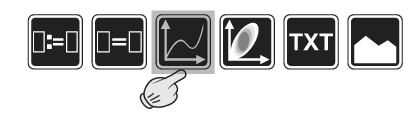
\includegraphics[width=0.45\textwidth]{graphics/how_to_use_fig8.png} \end{tabular}\end{center}

Aparece un panel con seis campos
vacíos. La función que se va a
graficar deberá ser puesta en el campo
medio-izquierdo y el argumento de la
función en el campo medio-inferior:
\begin{center}\begin{tabular}{c} 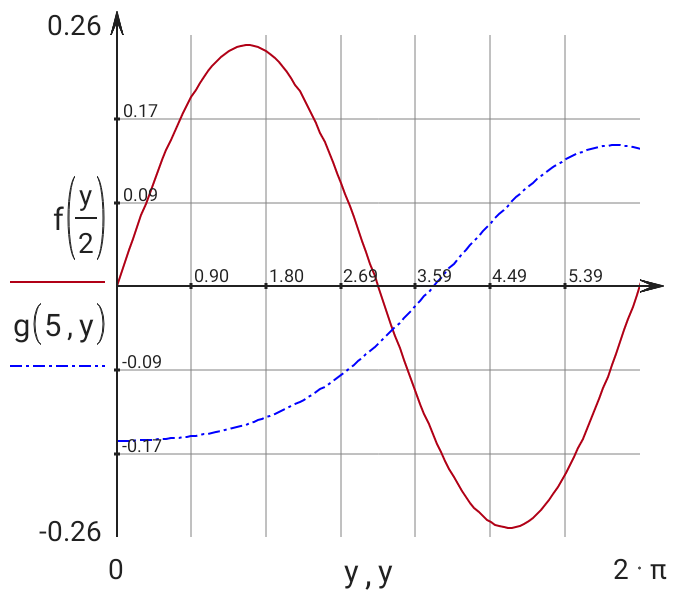
\includegraphics[width=0.45\textwidth]{graphics/how_to_use_fig9.png} \end{tabular}\end{center}

Para más detalles ver ''Gráfica de
funciones'' y ejemplos de ''Gráfica de
funciones polares'' del cajón de
navegación de aplicaciones.

\subsection{Gráfica tridimensional}

El elemento de la gráfica 3D muestra un
gráfico de una sola función que
depende de dos argumentos. Para crear
un gráfico de este tipo, utilice el
botón ''Nuevo elemento'' de la barra de
acciones o el botón ''Añadir gráfico
3D'' de la barra de herramientas:
\begin{center}\begin{tabular}{c} 
\includegraphics[width=0.45\textwidth]{graphics/how_to_use_fig10.png} \end{tabular}\end{center}
\begin{center}\begin{tabular}{cc}
  $x := \left[ -10,\, -9.5 \,..\, 10 \right]$ &
  $y := \left[ -10,\, -9.5 \,..\, 10 \right]$ \cr
\end{tabular}\end{center}
\begin{center}\begin{tabular}{c} 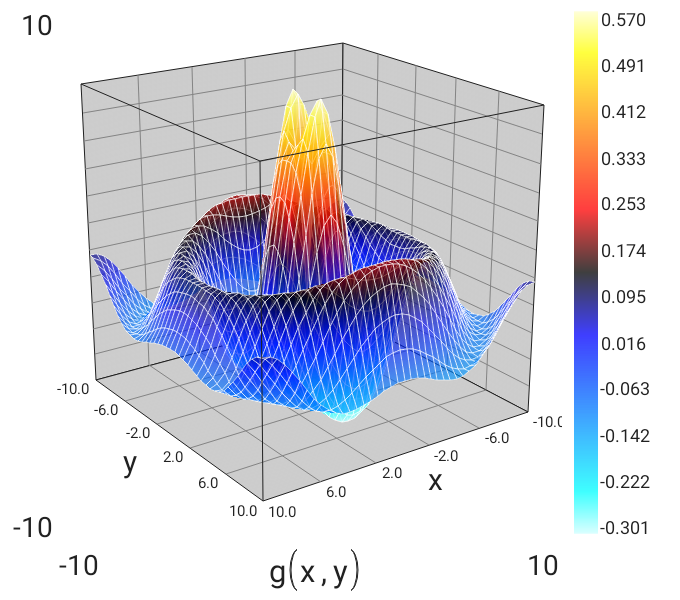
\includegraphics[width=0.45\textwidth]{graphics/how_to_use_fig11.png} \end{tabular}\end{center}

En el campo central-inferior, coloca el
nombre de la función o una ecuación
que contiene exactamente dos
intervalos previamente definidos. El
uso de una matriz también es posible:
\begin{center}\begin{tabular}{c} 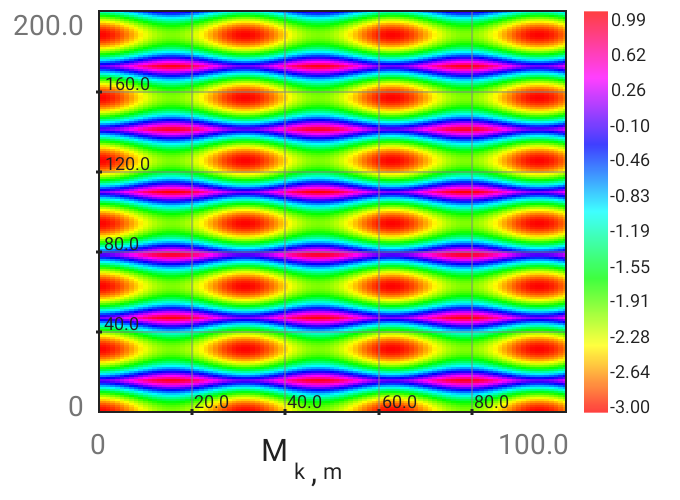
\includegraphics[width=0.45\textwidth]{graphics/how_to_use_fig12.png} \end{tabular}\end{center}

Para más detalles vea el ejemplo
''Gráfico 3D'' del cajón de navegación
de aplicaciones.

\subsection{Fragmento de texto}

El elemento de fragmento de texto
muestra un texto simple como este.
Para añadir un fragmento de texto,
utilice el botón ''Nuevo elemento'' de
la barra de acciones o el botón
''Añadir fragmento de texto'' de la
barra de herramientas:
\begin{center}\begin{tabular}{c} 
\includegraphics[width=0.45\textwidth]{graphics/how_to_use_fig13.png} \end{tabular}\end{center}

Si todo el texto dentro de un fragmento
es  seleccionado mediante el menú
contextual ''Seleccionar todo'',
aparecerá un botón flotante
''Propiedades del objeto'' en la parte
inferior derecha de la pantalla.

Si pulsa en este botón, aparecerá el
diálogo ''Propiedades de texto'', donde
podrá seleccionar el estilo de texto y
activar la numeración. Por ejemplo,
los títulos de este documento tienen
el estilo ''Subsección'' con la
numeración activada.

\subsection{Image}

También puedes insertar una imagen del
archivo de imágenes. Para hacerlo, usa
el botón ''Nuevo elemento'' de la barra
de acciones o el botón ''Añadir imagen
desde archivo'' de la barra de
herramientas:
\begin{center}\begin{tabular}{c} 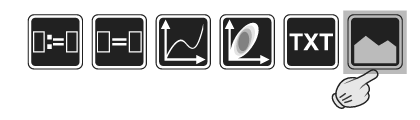
\includegraphics[width=0.45\textwidth]{graphics/how_to_use_fig14.png} \end{tabular}\end{center}

Aparecerá el diálogo '' Ajustes de
imagen''. Allí puede seleccionar un
archivo con la imagen que se va a
insertar y establecer el tamaño de
imagen necesario.

Los siguientes formatos de imagen son
soportados: png, bmp, gif, jpeg, svg.

Si activa el indicador ''Imagen
incrustada'' en el diálogo ''Ajustes de
imagen'', entonces la imagen se
incrustará directamente en el
documento. La imagen incrustada
operará dentro del único documento,
excepto en un archivo más grande.

Si el indicador ''Imagen incrustada'' no
está activado, el archivo de imagen
sólo será referenciado en lugar de
incrustarlo, es decir, su documento
vinculará al archivo de la imagen por
separado. En caso de que mueva su
documento por favor no olvide mover el
archivo de imagen también.

Puede cambiar las propiedades de una
imagen ya existente. Mantén presionado
en el área de la imagen hasta que
aparezca el botón flotante de
''Propiedades del objeto''. Si presiona
este botón, se mostrará un diálogo con
las propiedades de la imagen.

\section{Ejemplo: Gráfica de una función}
% This is auto-generated file: do not edit!
% Exported from microMathematics Plus, version 2.22.0


Este ejemplo demuestra cómo preparar y
ajustar una representación gráfica de
una función. por ejemplo, queremos
trazar tres diferentes funciones:
\begin{center}\begin{tabular}{c}
  $f(x) := 25 + 10 \cdot sin \left( \sqrt{ \left| x \right| } \right) $
\end{tabular}\end{center}
\begin{center}\begin{tabular}{c}
  $g(x) := \frac{2}{{e}^{ \left| x \right|  / 15}} \cdot f \left( x \cdot 50\right) $
\end{tabular}\end{center}
\begin{center}\begin{tabular}{c}
  $h(x) := min \left( f \left( x\right) ,\, g \left( x\right) \right) $
\end{tabular}\end{center}

El argumento de la función que
representa los valores x se tomarán
para puntos N dentro del intervalo
[x1, x2]:
\begin{center}\begin{tabular}{ccc}
  $N := 300$ &
  $x1 := -30$ &
  $x2 := 30$ \cr
\end{tabular}\end{center}
\begin{center}\begin{tabular}{c}
  $x := \left[ x1,\, x1 + \left( x2 - x1 \right) / N \,..\, x2 \right]$
\end{tabular}\end{center}

Una vez definidas las funciones y sus
argumentos se puede añadir el cuadro
de trazado mediante el botón ''Nuevo
elemento'' de la barra de acciones o el
botón ''Añadir gráfico de función'' de
la barra de herramientas:
\begin{center}\begin{tabular}{c} 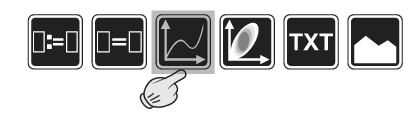
\includegraphics[width=0.45\textwidth]{graphics/function_plot_fig1.png} \end{tabular}\end{center}
\begin{center}\begin{tabular}{c} 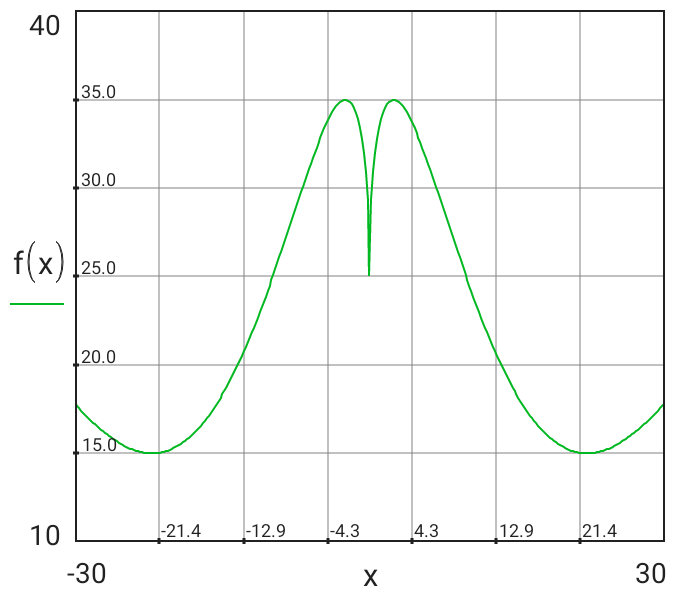
\includegraphics[width=0.45\textwidth]{graphics/function_plot_fig2.png} \end{tabular}\end{center}

La función que se graficará se pondrá
en el campo medio-izquierdo. También
puede ser una función incorporada o
previamente declarada así como una
expresión matemática que contiene
cualquier otro operador y función.

La entrada de la función, que
representa los valores x se pondrá en
el campo medio-inferior. Puede ser una
variable de tipo intervalo o una
expresión matemática que contiene una
variable de intervalo.

Los otros cuatro campos describen los
límites de la gráfica. Si estos
elementos permanecen vacíos, el
programa calculará los valores
correspondientes automáticamente. Sin
embargo, puede editar estos campos en
cualquier momento y poner allí los
valores que desee.

Puede graficar varias funciones en la
misma vista del gráfico. Para añadir
otra función, seleccione la función
(pulsando brevemente en el campo
medio-izquierdo) después de añadir
otra función y pulse el botón ''Añadir
nuevo argumento'' de la barra de
herramientas:
\begin{center}\begin{tabular}{c} 
\includegraphics[width=0.45\textwidth]{graphics/function_plot_fig3.png} \end{tabular}\end{center}
\begin{center}\begin{tabular}{c} 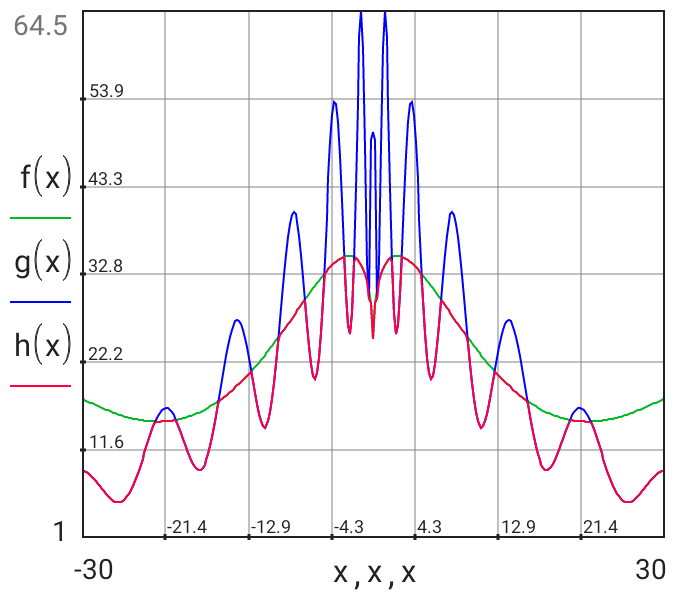
\includegraphics[width=0.45\textwidth]{graphics/function_plot_fig4.png} \end{tabular}\end{center}

Haciendo un largo toque en el centro
del área de la gráfica, aparecerá el
menú contextual y el botón flotante
''Propiedades de los objetos''.
\begin{center}\begin{tabular}{c} 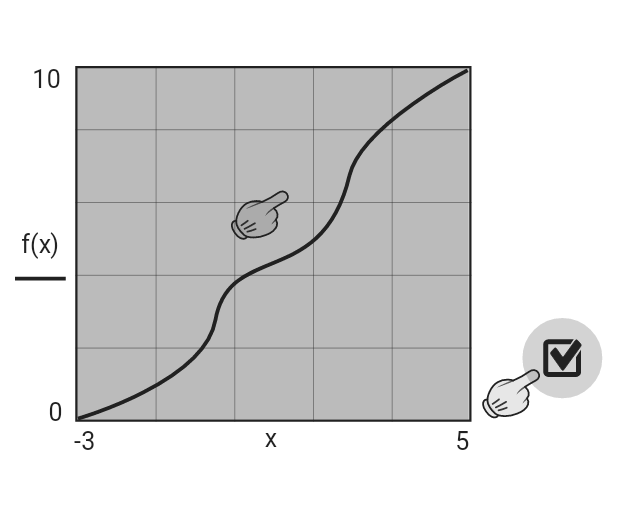
\includegraphics[width=0.45\textwidth]{graphics/function_plot_fig5.png} \end{tabular}\end{center}

Si presiona este botón flotante, se
mostará el diálogo de ''Ajustes de la
gráfica''. Aquí, puedes cambiar el
tamaño y el estilo del área de la
gráfica. Por ejemplo, el gráfico
cruzado se ve como esto:
\begin{center}\begin{tabular}{c} 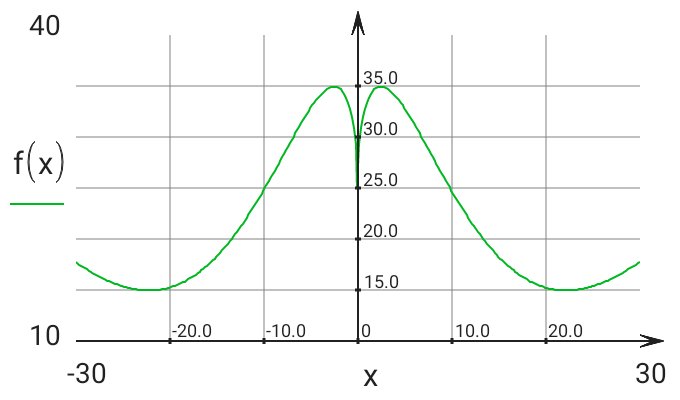
\includegraphics[width=0.45\textwidth]{graphics/function_plot_fig6.png} \end{tabular}\end{center}

También puedes cambiar la línea del
gráfico color, anchura y estilo en el
diálogo ''Ajustes de línea''. Aparece al
mantener presionado en la línea
marcada debajo del nombre de la
función a la izquierda de área de la
gráfica:
\begin{center}\begin{tabular}{c} 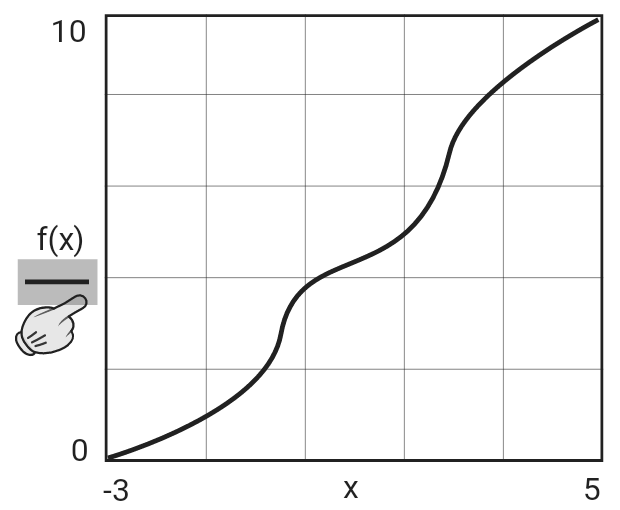
\includegraphics[width=0.45\textwidth]{graphics/function_plot_fig7.png} \end{tabular}\end{center}

Por ejemplo, podemos usar líneas
punteadas:
\begin{center}\begin{tabular}{c} 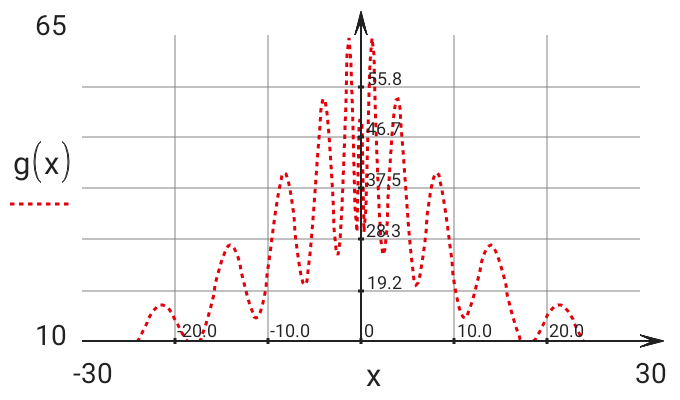
\includegraphics[width=0.45\textwidth]{graphics/function_plot_fig8.png} \end{tabular}\end{center}

El número de etiquetas de los ejes y la
línea de la cuadrícula color se puede
cambiar en el diálogo ''Ajustes de
cuadrícula''. Aparece al mantener
presionado en el espacio libre entre
el  valor mínimo de x (-30) y el
símbolo del argumento (x) o entre el
símbolo x junto al valor máximo x (30)
debajo del área de la gráfica
\begin{center}\begin{tabular}{c} 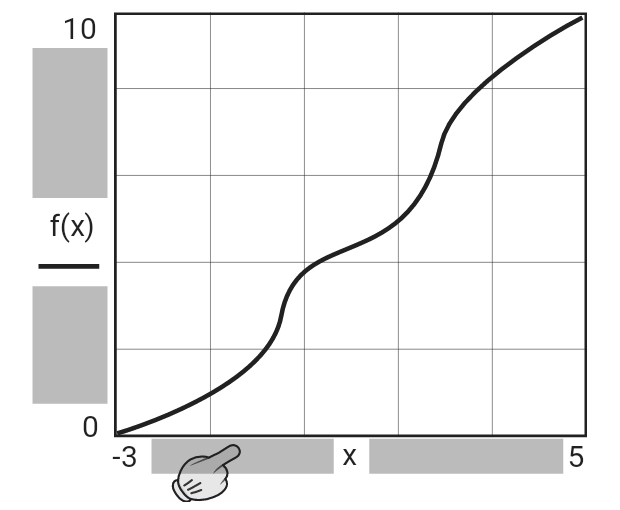
\includegraphics[width=0.45\textwidth]{graphics/function_plot_fig9.png} \end{tabular}\end{center}
\begin{center}\begin{tabular}{c} 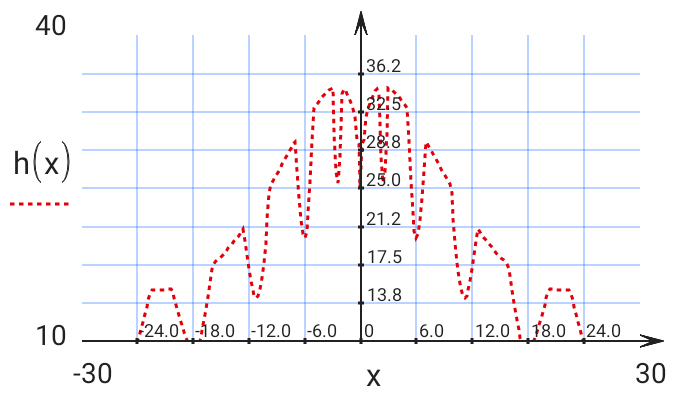
\includegraphics[width=0.45\textwidth]{graphics/function_plot_fig10.png} \end{tabular}\end{center}

Para ocultar la cuadrícula por completo
sólo hay que poner a cero el número de
líneas de la cuadrícula para ambos
ejes verticales y horizontales. Para
ocultar la cuadrícula por completo
sólo hay que poner a cero el número de
líneas de la cuadrícula para ambos
ejes verticales y horizontales.

\section{Ejemplo: Gráfica de una función polar}
% This is auto-generated file: do not edit!
% Exported from microMathematics Plus, version 2.22.0


Ahora trazamos varias funciones dadas
en el sistema de coordenadas polares.
Cada punto de este sistema está
determinado por una distancia r desde
el origen y el ángulo f desde el eje
x.
\begin{center}\begin{tabular}{c} 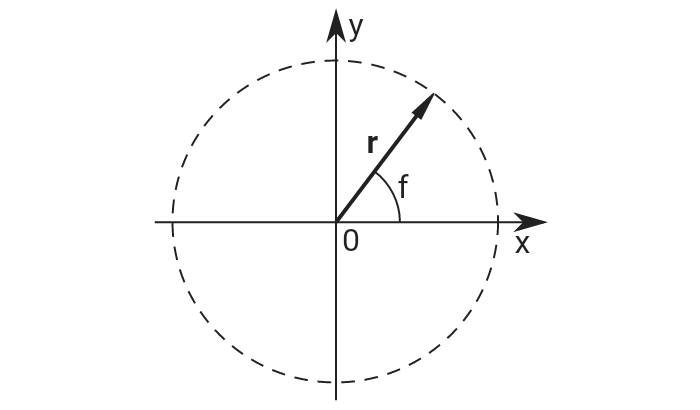
\includegraphics[width=0.45\textwidth]{graphics/polar_plot_fig1.png} \end{tabular}\end{center}

El ángulo f es nuestra variable
independiente que se cambia de la
siguiente manera:
\begin{center}\begin{tabular}{c}
  $f := \left[ 0.01,\, 0.05 \,..\, 300 \right]$
\end{tabular}\end{center}

La distancia r(f) es nuestra variable
dependiente. Teniendo un par de f y r,
podemos transformarla en las
coordenadas cartesianas x e y usando
funciones de seno y coseno:
\begin{center}\begin{tabular}{cc}
  $x(r) := r \cdot cos \left( f\right) $ &
  $y(r) := r \cdot sin \left( f\right) $ \cr
\end{tabular}\end{center}

\subsection{Un caracol}

Definiremos nuestra función polar en
tres pasos. La primera expresión
define una ''rueda'':
\begin{center}\begin{tabular}{ccc}
  $A := 1.1$ &
  $B := 1.271$ &
  $q := 2$ \cr
\end{tabular}\end{center}
\begin{center}\begin{tabular}{c}
  $r1(f) := A + 2 \cdot {sin \left( B \cdot f\right) }^{q}$
\end{tabular}\end{center}

Para trazar esta función, añadimos el
cuadro gráfico usando el botón ''Nuevo
elemento'' en la barra de acciones o el
botón ''Añadir gráfica de la función''
de la barra de herramientas:
\begin{center}\begin{tabular}{c} 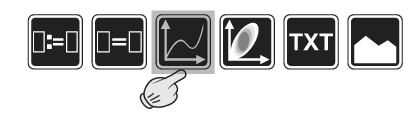
\includegraphics[width=0.45\textwidth]{graphics/polar_plot_fig2.png} \end{tabular}\end{center}

En lugar de f y r, usaremos aquí reglas
previamente definidas de la
transformación para x e y, donde r1(f)
se utiliza como un argumento simbólico
para estas reglas:
\begin{center}\begin{tabular}{c} 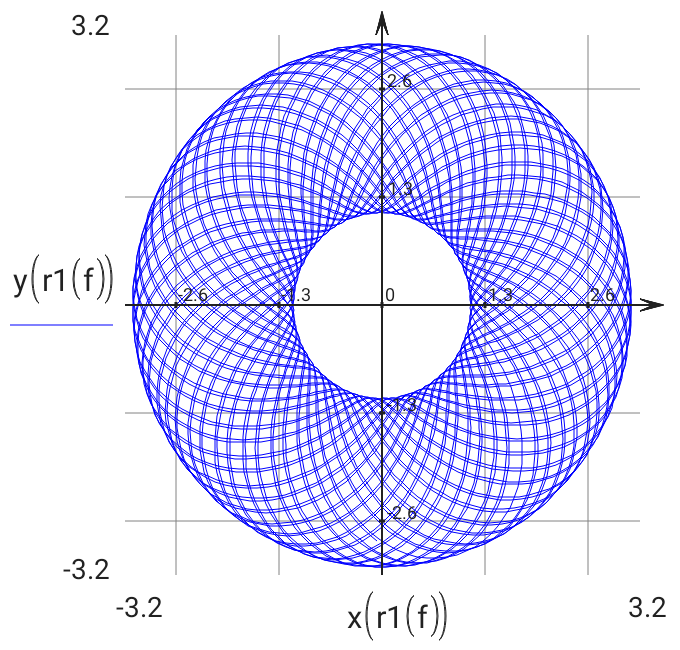
\includegraphics[width=0.45\textwidth]{graphics/polar_plot_fig3.png} \end{tabular}\end{center}

A continuación, podemos modificar esta
rueda a continuación:
\begin{center}\begin{tabular}{c}
  $r2(f) := A + 2 \cdot {sin \left( B \cdot f + 1 \cdot r1 \left( f\right) \right) }^{q}$
\end{tabular}\end{center}
\begin{center}\begin{tabular}{c} 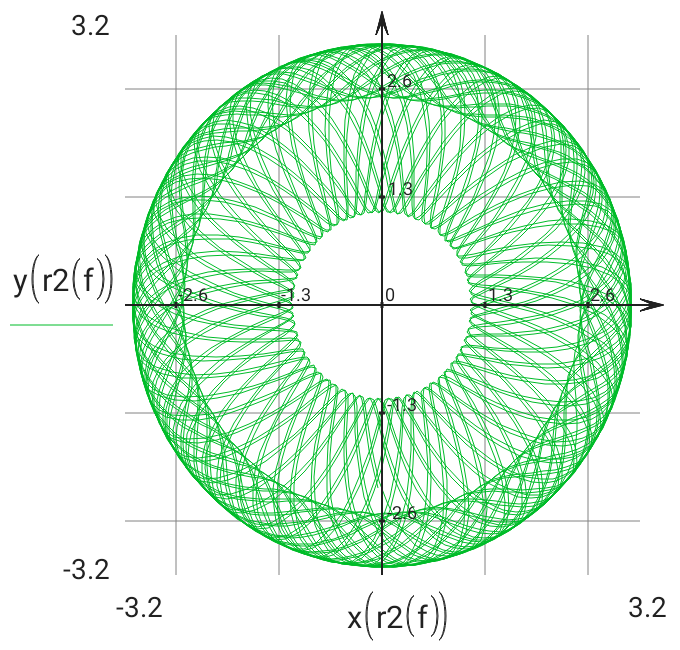
\includegraphics[width=0.45\textwidth]{graphics/polar_plot_fig4.png} \end{tabular}\end{center}

Finalmente, escalamos la última función
r2(f) usando un conversión de flotador
a número para parecer a una función de
paso. Como resultado, obtenemos un
bonito caracol:
\begin{center}\begin{tabular}{c}
  $r(f) := r2 \left( f\right)  \cdot floor \left( f\right)  / 10$
\end{tabular}\end{center}
\begin{center}\begin{tabular}{c} 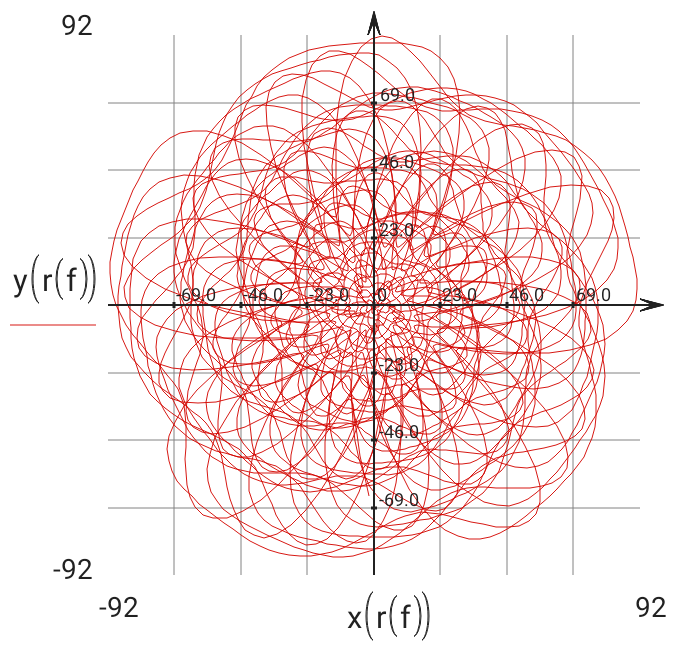
\includegraphics[width=0.45\textwidth]{graphics/polar_plot_fig5.png} \end{tabular}\end{center}

\subsection{Arce japonés}

El arce japonés es bien conocido por
sus atractivas formas de hojas y
colores. Tal hoja puede ser descrita
matemáticamente y trazada como una
curva en el sistema de coordenadas
polares:
\begin{center}\begin{tabular}{c}
  $f := \left[ 0.01,\, 0.02 \,..\, 100 \right]$
\end{tabular}\end{center}
\begin{center}\begin{tabular}{cc}
  $x(r) := r \cdot cos \left( f\right) $ &
  $y(r) := r \cdot sin \left( f\right) $ \cr
\end{tabular}\end{center}
\begin{center}\begin{tabular}{c}
  $s1(f) := \left( 1 + sin \left( f\right)  \right) \cdot \left( 1 - 0.9 \cdot  \left| sin \left( 4 \cdot f\right)  \right|  \right)$
\end{tabular}\end{center}
\begin{center}\begin{tabular}{c}
  $s2(f) := 0.9 + 0.05 \cdot cos \left( 200 \cdot f\right) $
\end{tabular}\end{center}
\begin{center}\begin{tabular}{c}
  $r(f) := floor \left( f\right)  \cdot s1 \left( f\right)  \cdot s2 \left( f\right)  + random \left( 2\right)  - 1$
\end{tabular}\end{center}
\begin{center}\begin{tabular}{c} 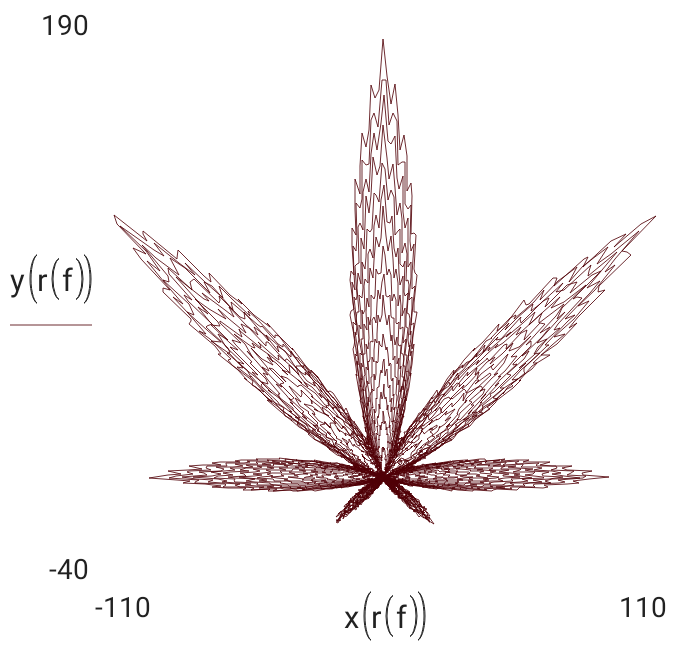
\includegraphics[width=0.45\textwidth]{graphics/polar_plot_fig6.png} \end{tabular}\end{center}

http://es.wikipedia.org/wiki/Acer\_palmatum

\section{Ejemplo: Gráfico 3D}
% This is auto-generated file: do not edit!
% Exported from microMathematics Plus, version 2.22.0


Este ejemplo muestra gráficos en 3D
para tres funciones diferentes de dos
variables.

Primero, definimos los intervalos para
los argumentos x e y. El intervalo
para el eje x depende del número de
puntos a lo largo del eje x y de los
valores mínimo y máximo, x1 y x2:
\begin{center}\begin{tabular}{ccc}
  $N := 300$ &
  $x1 := -2$ &
  $x2 := 2$ \cr
\end{tabular}\end{center}
\begin{center}\begin{tabular}{c}
  $x := \left[ x1,\, x1 +  \left| x2 - x1 \right|  / N \,..\, x2 \right]$
\end{tabular}\end{center}

El intervalo para el eje y está
definido análogamente:
\begin{center}\begin{tabular}{ccc}
  $M := 300$ &
  $y1 := -3$ &
  $y2 := 3$ \cr
\end{tabular}\end{center}
\begin{center}\begin{tabular}{c}
  $y := \left[ y1,\, y1 +  \left| y2 - y1 \right|  / M \,..\, y2 \right]$
\end{tabular}\end{center}

Por ejemplo, trazaremos una función
trigonométrica que es un producto del
seno y el coseno:
\begin{center}\begin{tabular}{c}
  $F(x,y) := sin \left( 3 \cdot {x}^{2}\right)  \cdot cos \left( {y}^{2}\right) $
\end{tabular}\end{center}

Para crear una vista en 3D, haga clic
en el botón ''Nuevo elemento'' de la
barra de acciones o en el botón
''Añadir gráfico 3D'' de la barra de
herramientas:
\begin{center}\begin{tabular}{c} 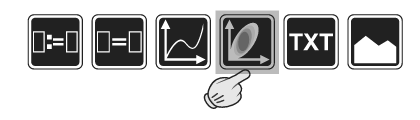
\includegraphics[width=0.45\textwidth]{graphics/three_d_plot_fig1.png} \end{tabular}\end{center}

Coloca el nombre de la función F(x,y)
en el campo central-inferior:
\begin{center}\begin{tabular}{c} 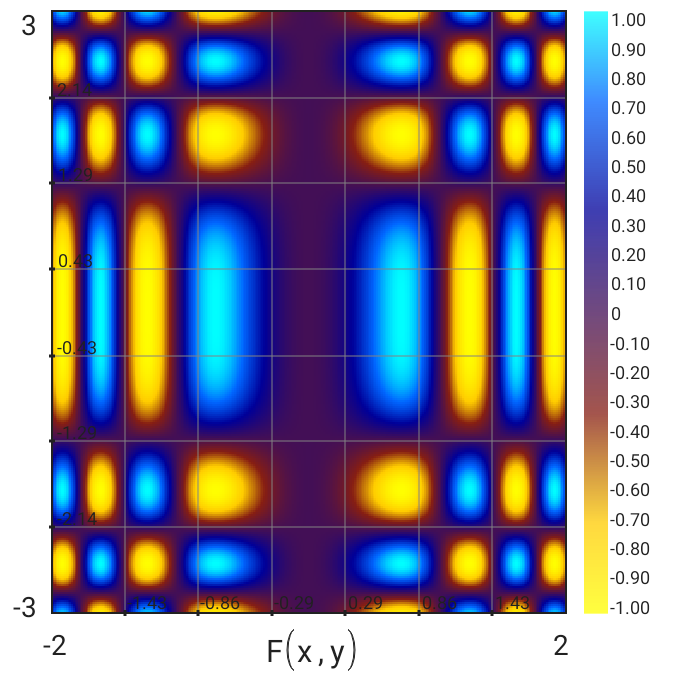
\includegraphics[width=0.45\textwidth]{graphics/three_d_plot_fig2.png} \end{tabular}\end{center}

Los límites del gráfico, el tamaño y el
estilo de los trazos, las etiquetas y
la cuadrícula se pueden ajustar por
analogía con el gráfico de funciones
utilizando el diálogo de ajustes de
gráficos (véase el ejemplo ''Gráfico de
la función'' de la caja de navegación
de aplicaciones para obtener más
detalles). Para abrir este cuadro de
diálogo, mantén presionado en el área
del gráfico hasta que aparezca el
botón flotante ''Propiedades del
objeto'', y luego pulse en este botón.

Adicionalmente, puede cambiar el
número de etiquetas a lo largo del eje
z y elegir la paleta de colores en el
cuadro de diálogo ''Ajustes de color de
la tabla''. Este diálogo aparece al
mantener presionado en la barra del
eje z a la derecha del área del
gráfico principal.
\begin{center}\begin{tabular}{c}
  $R(x,y) := sin \left( 5 \cdot {x}^{2} \cdot \left( y - x \right)\right) $
\end{tabular}\end{center}
\begin{center}\begin{tabular}{c} 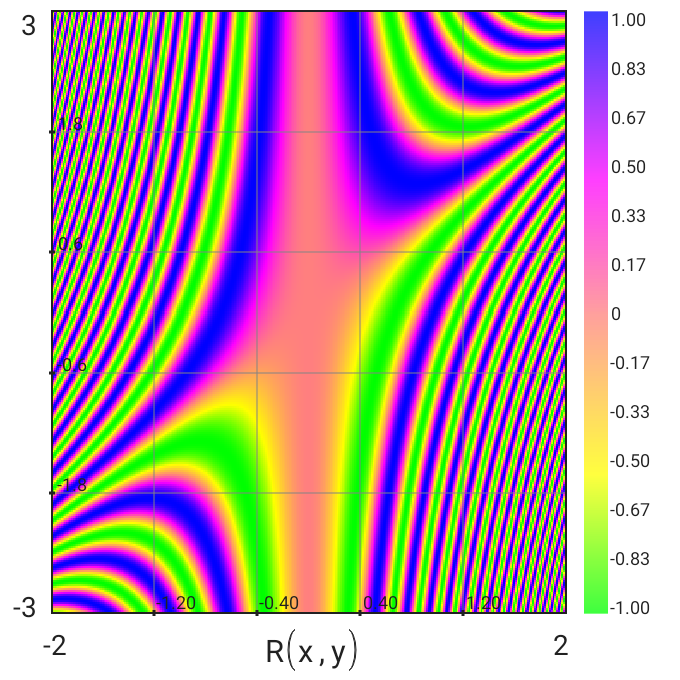
\includegraphics[width=0.45\textwidth]{graphics/three_d_plot_fig3.png} \end{tabular}\end{center}

También se puede trazar una función de
dos argumentos como una superficie en
el espacio 3D. Este modo puede
activarse en el cuadro de diálogo
''Ajustes de la gráfica'' que aparece si
se pulsa en el botón flotante
''Propiedades del objeto'' después de
hacer un largo pulso en el área del
trazado. Trazamos la siguiente
función, utilizando matrices para
mejorar el tiempo de cálculo:
\begin{center}\begin{tabular}{cccc}
  $N := 100$ &
  $n := \left[ 0,\, 1 \,..\, N \right]$ &
  $x1 := -15$ &
  $x2 := 15$ \cr
\end{tabular}\end{center}
\begin{center}\begin{tabular}{cccc}
  $M := 100$ &
  $m := \left[ 0,\, 1 \,..\, M \right]$ &
  $y1 := -15$ &
  $y2 := 15$ \cr
\end{tabular}\end{center}
\begin{center}\begin{tabular}{c}
  $x_{n}  := {\left( x1 +  \left( x2 - x1\right)  \cdot n / N \right)}^{2}$
\end{tabular}\end{center}
\begin{center}\begin{tabular}{c}
  $y_{m}  := {\left( y1 +  \left( y2 - y1\right)  \cdot m / M \right)}^{2}$
\end{tabular}\end{center}
\begin{center}\begin{tabular}{c}
  $r_{n,\, m}  := 0.04 \cdot x_{n}  + 0.02 \cdot y_{m} $
\end{tabular}\end{center}
\begin{center}\begin{tabular}{c}
  $t_{n,\, m}  := \left( x_{n}  + 0.05 \cdot y_{m}  \right) \cdot exp \left( 1 - r_{n,\, m} \right) $
\end{tabular}\end{center}
\begin{center}\begin{tabular}{c}
  $F_{n,\, m}  := \frac{sin \left( x_{n}  + 0.1 \cdot y_{m} \right) }{0.15 + r_{n,\, m} } + \frac{t_{n,\, m} }{10}$
\end{tabular}\end{center}
\begin{center}\begin{tabular}{c} 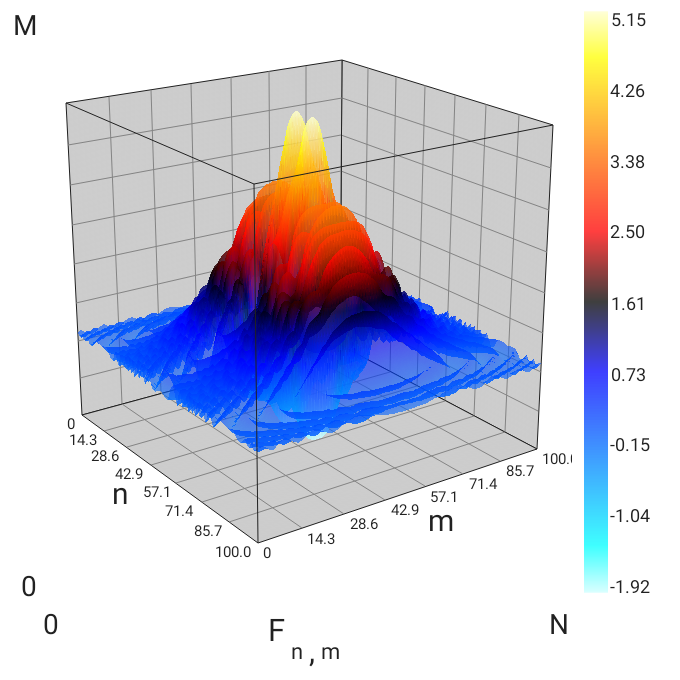
\includegraphics[width=0.45\textwidth]{graphics/three_d_plot_fig4.png} \end{tabular}\end{center}

Para el gráfico de la superficie, hay
ajustes adicionales presentados en el
diálogo ''Ajustes de la gráfica''.
Puedes elegir si se muestran las
líneas de malla, seleccionar la
opacidad para el color de la malla,
definir los ángulos de rotación y
elevación del cuadro de trazado. Por
ejemplo, la superficie anterior
trazada con otros ángulos de rotación
y elevación se ve así: 
\begin{center}\begin{tabular}{c} 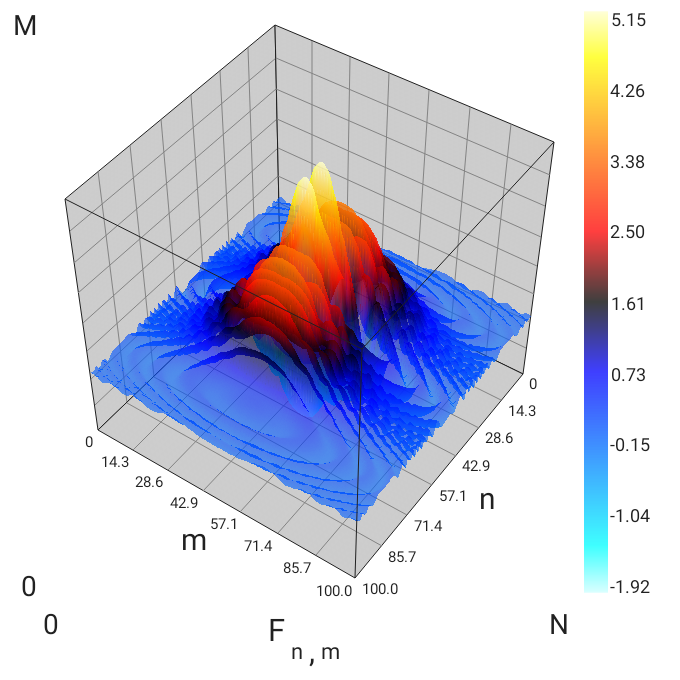
\includegraphics[width=0.45\textwidth]{graphics/three_d_plot_fig5.png} \end{tabular}\end{center}

\section{Ejemplo: Series e integrales}
% This is auto-generated file: do not edit!
% Exported from microMathematics Plus, version 2.20.0


Este ejemplo demuestra cómo calcular
series e integrales.

\subsection{Serie de Taylor}

En matemáticas, la serie de Taylor es
una representación de una función como
una suma infinita de términos que se
calculan a partir de los valores de
las derivadas de la función en un solo
punto.

Por ejemplo, Ts(x,N) es la expansión
de Taylor en función del argumento x y
del número de términos N:
\begin{center}\begin{tabular}{c}
  $Ts(x,N) := \displaystyle\sum_{n=0}^{N} \frac{{ \left( -1\right) }^{n}}{\left( 2 \cdot n \right)! } \cdot {x}^{2 \cdot n}$
\end{tabular}\end{center}

Esta expansión se aproxima a la función
coseno:
\begin{center}\begin{tabular}{c}
  $s(x) := cos \left( x\right) $
\end{tabular}\end{center}

Si trazamos ambas funciones juntas para
el mismo intervalo, ambas parecen
iguales:
\begin{center}\begin{tabular}{c}
  $x := \left[ 0,\, 0.1 \,..\, 2 \cdot {\pi} \right]$
\end{tabular}\end{center}
\begin{center}\begin{tabular}{c} 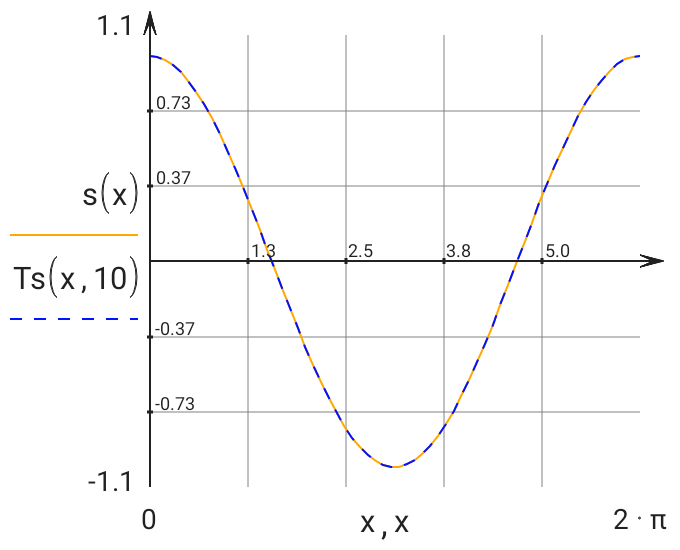
\includegraphics[width=0.45\textwidth]{graphics/series_and_integrals_fig1.png} \end{tabular}\end{center}

Sin embargo, hay un error numérico
debido al número limitado de términos
de aproximación N. La siguiente
función $\Delta$(x,N) describe este error:
\begin{center}\begin{tabular}{c}
  ${\Delta}(x,N) :=  \left| s \left( x\right)  - Ts \left( x,\, N\right)  \right| $
\end{tabular}\end{center}

Podemos graficar esta función en
coordenadas logarítmicas y ver que el
error numérico disminuirá si
introducimos más términos en la suma
de Taylor:
\begin{center}\begin{tabular}{c}
  $N := \left[ 3,\, 4 \,..\, 13 \right]$
\end{tabular}\end{center}
\begin{center}\begin{tabular}{c} 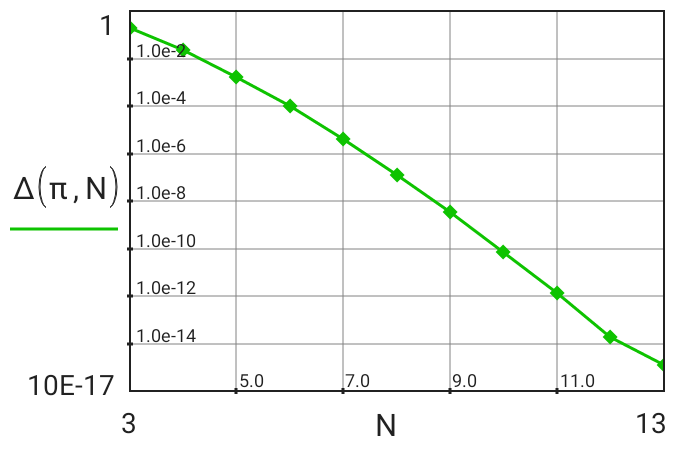
\includegraphics[width=0.45\textwidth]{graphics/series_and_integrals_fig2.png} \end{tabular}\end{center}

\subsection{Serie de binomios}

Consideremos esta función de poder:
\begin{center}\begin{tabular}{c}
  $f(x,{\alpha}) := {\left( 1 + x \right)}^{{\alpha}}$
\end{tabular}\end{center}

Esta función puede ser aproximada
usando serie de binomios:
\begin{center}\begin{tabular}{c}
  $Tf(x,{\alpha},N) := \displaystyle\sum_{n=0}^{N}  \left( \displaystyle\prod_{k=1}^{n} \frac{{\alpha} - k + 1}{k}\right)  \cdot {x}^{n}$
\end{tabular}\end{center}

También podemos graficar ambas
funciones (la función de potencia dada
y su aproximación) juntas en la misma
gráfica:
\begin{center}\begin{tabular}{c} 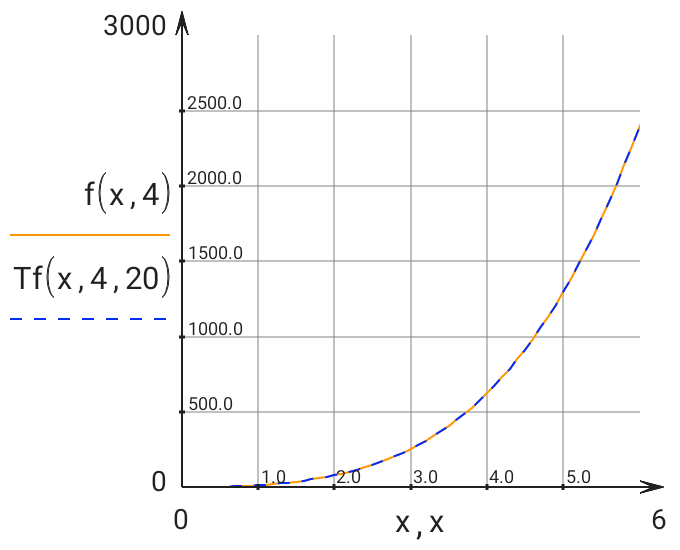
\includegraphics[width=0.45\textwidth]{graphics/series_and_integrals_fig3.png} \end{tabular}\end{center}

\subsection{Integrales}

También es posible calcular una
integral definida numéricamente usando
el método de Simpson. Por ejemplo,
podemos calcular la integral usando el
elemento ''Añadir vista de resultados'':
\begin{center}\begin{tabular}{c}
  $\displaystyle\int_{0}^{3 \cdot pi / 2}{cos \left( \frac{2 \cdot x}{9}\right) }^{-2}\, dx = 7.79423$
\end{tabular}\end{center}

La solución analítica es
\begin{center}\begin{tabular}{ccc}
  $I := \frac{9 \cdot \sqrt{3} }{2}$ &
  ,    &
  $I = 7.79423$ \cr
\end{tabular}\end{center}

El error numérico puede calcularse
como:
\begin{center}\begin{tabular}{c}
  $\displaystyle\int_{0}^{3 \cdot pi / 2}{cos \left( \frac{2 \cdot x}{9}\right) }^{-2}\, dx - I = 4.26681E-9$
\end{tabular}\end{center}

Este error depende del valor ''Cifras
significativas en el resultado'' que se
puede cambiar en el cuadro de diálogo
''Ajustes del documento'' disponible en
la barra de acciones:
\begin{center}\begin{tabular}{c} 
\includegraphics[width=0.45\textwidth]{graphics/series_and_integrals_fig4.png} \end{tabular}\end{center}

Si este valor aumenta, el umbral que
controla la precisión del método
Simpson también aumentará.

\section{Sobre microMathematics Plus}
% This is the second part of the file about_micromath.tex
\subsection{Autores}

\begin{enumerate}
\item Mikhail Kulesh,
mikhail.kulesh@gmail.com

\item Caio Roberto Ramos da Silva
(Brazilian Portuguese translation),
caiorrs@gmail.com

\item Yubin Hsu
(Chinese translation),
yubin.taiwan@gmail.com

\item Linsui
(Chinese translation),
linsui555@gmail.com

\item Diego Sanguinetti
(Spanish translation)
\end{enumerate}

\subsection{Icono de la app}

El icono de la aplicación se genera a partir de la siguiente
función definida en el
sistema de coordenadas polares:
\begin{center}\begin{tabular}{c}
                $f := \left[ 0.01,\, 0.03 \,..\, 150 \right]$
\end{tabular}\end{center}
\begin{center}\begin{tabular}{c}
                $s(f) := 4 + sin \left( 5 \cdot f\right)  + \frac{sin \left( 10 \cdot f\right) }{2} + \frac{sin \left( 60 \cdot f\right) }{6}$
\end{tabular}\end{center}
\begin{center}\begin{tabular}{c}
                $r(f) := 0.9 \cdot \left( 1 + f / 50 \right) \cdot s \left( f\right) $
\end{tabular}\end{center}
\begin{center}\begin{tabular}{c}
                $x(f) := r \left( f\right)  \cdot cos \left( f\right) $
\end{tabular}\end{center}
\begin{center}\begin{tabular}{c}
                $y(f) := r \left( f\right)  \cdot sin \left( f\right) $
\end{tabular}\end{center}
\begin{center}\begin{tabular}{c} 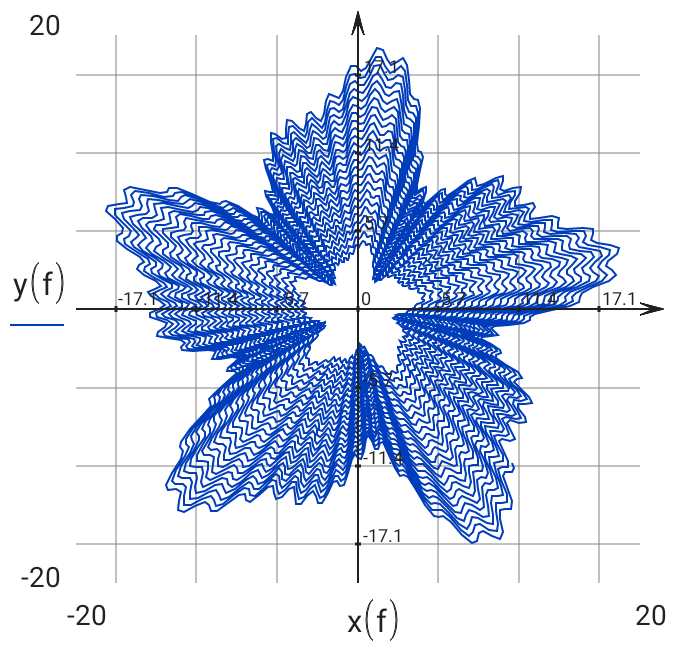
\includegraphics[width=0.45\textwidth]{graphics/about_micromath_fig1.png} \end{tabular}\end{center}

2014-2020, Bremen, Alemania
\end{document}